\section{Let There Be Light}

La société Let There Be Light (ou LTBL) est une société qui réalise des dispositifs interactifs pour l'événementiel, la communication et la culture.
Elle fut fondée en 2014 par Benjamin \bsc{Petit} et Antoine \bsc{Vanel} sous le nom de Beam'Art.
En 2016, elle change de nom et de statut pour devenir l'entreprise que l'on connaît aujourd'hui.
Actuellement, M. \bsc{Petit} en est le seul dirigeant et emploi 2 personnes.

\subsection{Structure}

Let There Be Light est un partenaire de la société Vendredi 4.
Vendredi 4 est une société de communication spécialisée dans l'interaction.
Les contrats sont obtenus par Sylvie \bsc{Madamour}, la charte graphique du projet est alors composée par Vendredi 4.
LTBL intervient sur l'intégration de cette charte graphique dans les installations interactives dans des salons ou des showrooms.

Les équipes de Vendredi 4 et de LTBL sont assez réduites.
L'effectif de Vendredi 4 est de 3 employé quand LTBL compte un unique employé (Benjamin \bsc{Petit}) et deux consultants : Corentin \bsc{Limoge} et Alexander \bsc{Feller}.

\begin{figure}[h]
    \centering
    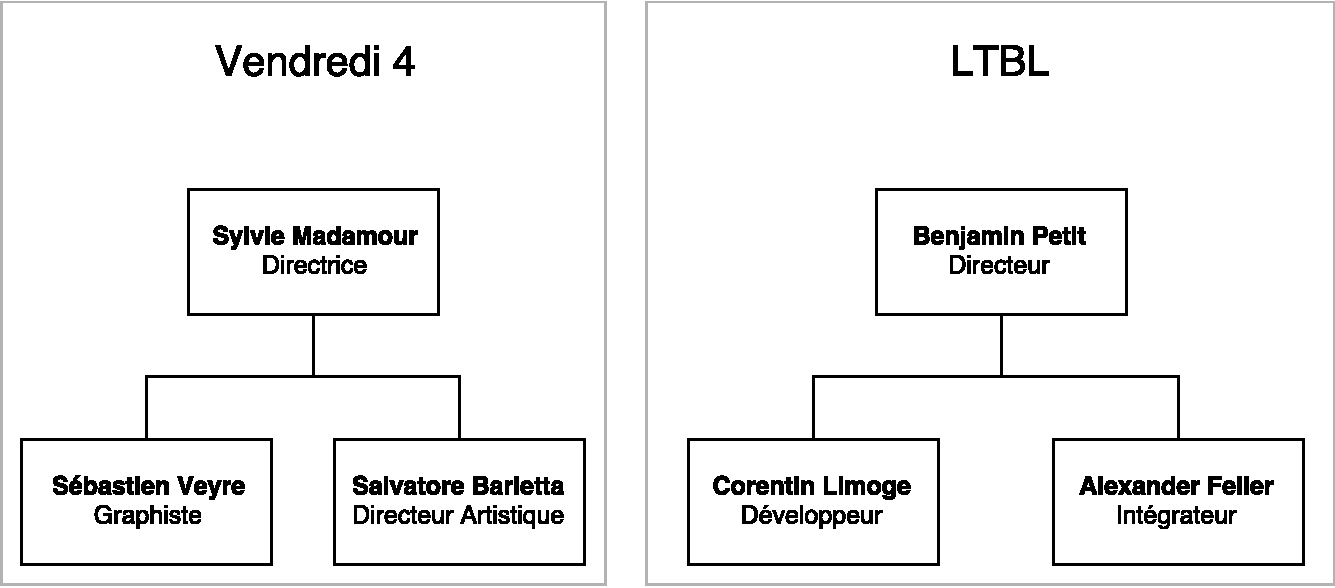
\includegraphics[scale=0.7]{img/Structure-LTBL.pdf}
    \caption{Structure de LTBL et Vendredi 4}
\end{figure}

Les deux entreprises sont très liées, elles partagent les mêmes locaux et communiquent beaucoup ensemble sur les projets en cours et à venir.

\subsection{Projets}

Les deux entreprises travaillent ensemble pour proposer des services suivants :

\begin{itemize}
    \item Conseils techniques
    \item Conseils en interaction
    \item Design graphique
    \item Développement d'applications interactives
    \item Installations
\end{itemize}

Ainsi, les deux entreprises peuvent suivre la production d'une application interactive de sa conception jusqu'à son installation.

\clearpage

Les projets suivis par LTBL sont les suivants :

\paragraph{Dispositifs de présentation interactifs} le plus souvent utilisés dans les salons et showrooms, les dispositifs interactifs permettent une présentation des produits de manière esthétique.
L'objectif de LTBL est donc de concevoir cette installation.
Cela passe par la conception du système physique est des composants requis mais aussi par la conception et le développement de l'interface utilisateur qui doit être réactive et esthétique.
La majorité de ce type de projet est la présentation d'informations sur un produit sur un écran tactile

\paragraph{Vidéo Mapping} Le plus souvent présenté lors d'événements, le vidéo mapping consiste en la projection d'une image déformée sur une structure pouvant être un bâtiment ou une installation spécifique.
Cette image utilise une représentation de la structure pour se déformer et épouser sa forme lors de la projection.
Ce type d'installation permet, au travers de jeux de lumière et d'illusions, de donner vie à la structure ou au bâtiment.
On retrouve ce type d'installation à la fête des Lumières de Lyon par exemple.

\paragraph{Conseils techniques ou en interaction} Fort de son expérience dans le domaine de l'interactivité, LTBL peut aussi donner des conseils en interactivité dans le cadre de projets cités plus haut.

\paragraph{Fête des Lumières} La fête des Lumières est une manifestation Lyonnaise prenant place aux endroits importants de la ville.
Cette fête met en lumière de nombreuses installations lumineuses et interactives.
Chaque année, LTBL peut proposer un projet d'installation en rapport avec un bâtiment de la ville sur lequel s'installer.
Ce projet est alors évalué et est accepté ou non en fonction de la faisabilité, l'esthétique et le coût de l'installation.